% JuliaCon proceedings template
\documentclass{juliacon}
\usepackage{amsmath}
\setcounter{page}{1}

\begin{document}

% **************GENERATED FILE, DO NOT EDIT**************

\title{Probabilistic Biostatistics with Julia}

\author[1]{Jeffrey A. Mills}
\author[1, 2]{Jeffrey R. Strawn}
\affil[1]{University of Cincinnati}
\affil[2]{Cincinnati Children's Hospital}

\keywords{Julia, Bayesian methods, Meta-analyses, Biostatistics, Randomized Controlled Trial}

\maketitle

\begin{abstract}

Medical research requires statistical tools that are both sophisticated and powerful enough to address complex inferential problems, as well as intuitive and user-friendly enough to not require advanced statistical and programming expertise.  Combining Julia with the Bayesian MCMC machinery addresses this need. Examples of Bayesian probabilistic biostatistics in Julia, including Bayesian adaptive trial design, sequential analysis of randomized controlled trials, and Bayesian hierarchical modeling for a meta-analysis are presented.  These examples illustrate the application of a sophisticatedly simple approach to statistical analysis and modeling for clinical research.

\end{abstract}

\section{Introduction}

Julia is widely recognized as a solution to “the two-language problem”: it is both fast and efficient (performance), and easy to use (user friendliness)\cite{bezanson2017julia}.  Additionally, using the Bayesian MCMC machinery in Julia solves “the two field problem”: clinical researchers often need expertise in both medicine and in statistical computing. As those conducting and funding clinical randomized controlled trials (RCTs) recognize the high costs of these studies (e.g., medication expense, time required, and potential exposure of patients to ineffective treatments), there has been greater enthusiasm for (1) improving statistical analytic methods for RCTs, and 2) using evidence-based methods to examine existing naturalistically collected clinical data to inform clinical practice without the need for RCTs. Thus, there is an urgent need to provide statistical tools to clinician-researchers that are intuitive and easy to use, yet sophisticated and powerful enough to answer questions that simpler methods cannot.
\vskip 6pt
The Bayesian machinery of posterior simulation and Markov chain Monte Carlo (MCMC) methods together with Julia offer a solution to this “two-field problem”. This enables exact small sample inference and hypothesis testing for complex models without requiring the restrictive assumptions necessary to obtain analytical tractability, and facilitates the analysis of complex models with basic statistical concepts: frequency distributions, density plots, means, medians, modes, standard deviations, quantiles, and posterior density ratios\cite{Mills2019}. 
\vskip 6pt
This paper presents examples from our research developing and applying Bayesian probabilistic approaches to inference and testing in RCTs\cite{Mills2019, Strawn2019, Strawn2018, Strawn2017, Strawn2018a}. Our approach leverages posterior simulation and MCMC methods which, being recursive, require efficient looping, so most available R packages rely on C++ code.  This leads to the need to either code in C++ or something similar, or rely on a black box package.  Julia offers a user-friendly coding experience similar to python, matlab or R, and many packages that, being written in Julia, allow one to examine and learn from the source code.  We are currently developing our own package, BayesTesting.jl\cite{Mills2018}, along with taking advantage of several Julia packages (e.g. Distributions.jl, DataFrames.jl, CSV.jl and Turing.jl) to apply MCMC and hierarchical models to conduct analyses and meta-analyses of data from RCTs\cite{Strawn2019}.

\section{Moving Hypothesis Testing Forward}
\label{sec:hypothesistest}

\begin{quote}
	At some future time trials may be evaluated using fully Bayesian notions of utilities and decisions ... which would enable designs to be built that do not violate the Likelihood Principle or Bayesian notions.  But currently, the regulatory structure is such that confirmatory trials are usually judged and evaluated using Type I error\cite{Berry20ll}, p.220-221.
\end{quote}
\vskip 6pt
Despite widespread criticism of p-values\cite{Berry2017}, the ``$p \le 0.05$ is ‘statistically significant’, $p > 0.05$ is not'' is an iron law for publishing in leading journals in many fields\cite{Wass2019}. In general, you cannot successfully publish applied science without precise hypothesis testing.  Statisticians, especially Bayesians, argue against that approach, but there is too much institutional inertia towards the use of $p$-values as `proper’ applied science\cite{Wass2019}.  At the very least, a bridge from `pure’ hypothesis testing to a more complete Bayesian analysis is needed.
\vskip 6pt
The comparison of means from two samples provides a canonical example. Suppose we have samples from two different treatments, $x_1$ and $x_2$, and wish to evaluate whether there is any evidence of a difference in average treatment effect (ATE).  This is equivalent to evaluating the precise vs. composite hypotheses,  
\begin{equation} 
H_0: \delta = 0, \; \; H_1: \delta \ne 0. 
\label{eq:hoh1}
\end{equation}
where $\delta = \mu_1 - \mu_2$, and $\mu_j$ is the ATE for treatment $j$.

Appealing to the Central Limit Theorem and the Principle of Maximum Entropy provides strong justification for assuming that the distribution of the sample mean, $\bar{x}_j$, for each sample is Gaussian, 
\begin{equation}
\bar{x}_j \sim N(\mu_j,\sigma_j^2/n_j ), \; \;    j=1,2,
\label{eq:xbar}
\end{equation}
where $\mu_j$ and $\sigma_j^2$ are the unknown population mean and variance of $x_j$, and $n_j$ is the number of observations in sample $x_j$. Adopting uninformative priors for the mean and variance leads to conditional posterior densities,
\begin{equation}
\mu_j | \sigma_j,x_j \sim N(\bar{x}_j, \sigma_j^2 /n),
\label{eq:muj}
\end{equation}
\begin{equation}
\sigma_j^2|x_j \sim IG((n_j-1)/2,(n_js_j^2)/2) = Inv-\chi^2(n_j-1,s_j^2).
\label{eq:sigmaj}
\end{equation}
where $s_j^2$ is the sample variance \cite{Gelman2004}. This is as far as we need to go analytically.  The rest of the problem can be solved numerically (though one more step is easily taken in this case, leading to a Student-t marginal posterior density for $\mu_j$ with posterior mean $\bar{x}_j$, variance $s_j^2/n$, and degrees of freedom $n_j-1$).
\vskip 6pt
Obtaining $M$ draws from these conditional distributions provides pseudo-samples from the marginal posteriors for $\mu$ and $\sigma^2$ (or drawing directly from the Student-t marginal posterior for $\mu$).  We then obtain an MCMC pseudo-sample of size $M$ from the posterior distribution of $\delta$, $\delta^{(m)} = \mu_1^{(m)} - \mu_2^{(m)},$ $m = 1,...,M$.  In this way, posteriors for any function of the parameters are available, such as differences in differences and ratios. For example, we often wish to compare two treatments to placebo, then to each other, which is accomplished by obtaining $\Delta^{(m)} = \delta_1^{(m)} - \delta_2^{(m)}$. While the analytical distribution of $\Delta$ is unknown and asymptotic approximations require unrealistic assumptions,  MCMC sampling allows the exact small sample posterior density to be approximated arbitrarily closely as $M$ is increased. The rest of the analysis requires only knowledge of basic statistics: plotting the density of the MCMC draws, computing summary statistics, and testing hypotheses.   Note that this addresses the Behrens-Fisher problem of testing the difference between the means of two populations when the variances of the two populations are not assumed either known or equal\cite{Ramos2010}.  Differing sample sizes for each group are also allowed.  Correlation across samples and other model extensions are straightforward.
\vskip 6pt
To test the hypotheses in (\ref{eq:hoh1}) we evaluate the posterior density ratio, PDR, (or `posterior odds') against $H_0$, by evaluating the MCMC posterior density for $\delta$ at the value in the null hypothesis and at the mode.  For treatment samples $x_1$ and $x_2$ the PDR is,
\begin{equation}
PDR(\delta = 0|x_1, x_2) = \frac{p(\delta=\delta_{MAP}|x_1,x_2)}{p(\delta=0|x_1,x_2)},
\label{eq:odds}
\end{equation}
where $\delta_{MAP}$ is the maximum a posteriori estimate of $\delta$.
We can also compute posterior tail probabilities (one-sided `Bayesian $p$-values'), from the MCMC sample,
\begin{equation}
p\text{-value} = \min{\left[P(\delta \le 0|x_1, x_2),P(\delta \ge 0|x_1, x_2)\right]},
\label{eq:pval}
\end{equation} 
$$P(\delta \le 0|x_1, x_2) =  \frac{\sum_{m=1}^M I(\delta^{(m)} \le 0) }  {M},$$
$$P(\delta \ge 0|x_1, x_2) =  \frac{\sum_{m=1}^M I(\delta^{(m)} \ge 0) }  {M},$$
where the indicator function $I(.) = 1$ if the condition is true, $0$ otherwise. These same formulas can be used to evaluate hypotheses concerning other quantities of interest, such as $\Delta$. The PDR for joint hypotheses (suppose $\delta$ is a vector of parameters) can readily be evaluated using Rao-Blackwellization\cite{Mills2018,Mills2019}.

\section{Bayesian adaptive trial design and sequential analysis}
The Bayesian machinery described above can be employed to perform adaptive trial design and sequential analysis of RCTs. In this context, the Bayesian approach offers the advantage of no statistical requirement for a stopping rule. Though other reasons for a stopping rule are important, such as funding and avoiding bias due to stopping when a test critical value is just reached, a sequential analysis minimizes costs, time and the number of patients exposed to inferior treatment. Further, there is no satisfactory frequentist differences of differences analysis without restrictive assumptions. The analytical sampling distributions are unknown and intractable; asymptotic assumptions are invalid with small samples; and there may be other constraints (e.g., boundary conditions). Bootstrapping is also inferior due to the small sample sizes. The commonly used Welch t-test represents an ad hoc attempt to deal with different variances across samples that does not perform well in simulations\cite{Mills2019}.  Importantly, these issues are resolved by the Bayesian machinery.
\vskip 6pt
In previous work\cite{Strawn2018,Mills2019}, data from a federally-funded NIH trial of pediatric anxiety disorders (Child/Adolescent Anxiety Multimodal Study [CAMS], N=488) were analyzed to validate the proposed methodology and to examine treatment and placebo responses. In CAMS, youth, aged 7-17 (mean age: 10.7 years) with generalized, separation and$/$or social anxiety disorders, were randomized (2:2:2:1) to cognitive behavioral therapy (CBT, n=139), a selective serotonin reuptake inhibitor (SSRI), sertraline (SRT, n=133), SRT+CBT (n=140), or pill placebo (PBO, n=76).
% insert pars_difference_sequential.png
% pars_difference_sequential.png
\vskip 6pt
The following example sequentially analyzes the data for the combined treatment SRT+CBT relative to PBO using Bayesian updating.  To evaluate the hypothesis in (\ref{eq:hoh1}) where $\mu_1$ is the ATE of SRT+CBT and $\mu_2$ is the ATE of PBO. Starting with a sample of 12 (8 treated, 4 placebo), the posterior density was updated with each additional 6 observations (4 treated:2 placebo).  The sequence of posteriors as $n$ is increased for the difference in ATE between SRT+CBT and PBO is shown in Figure~\ref{fig:pars_diff}, and the PDR giving posterior odds against the null hypothesis (\ref{eq:odds}), posterior probability that the difference is greater than zero (\ref{eq:pval}), and two sided $p$-value ($\approx 2\times p(\delta \ge 0)$) are given in Table \ref{tab:seq}.

\begin{figure}[t]
	\centerline{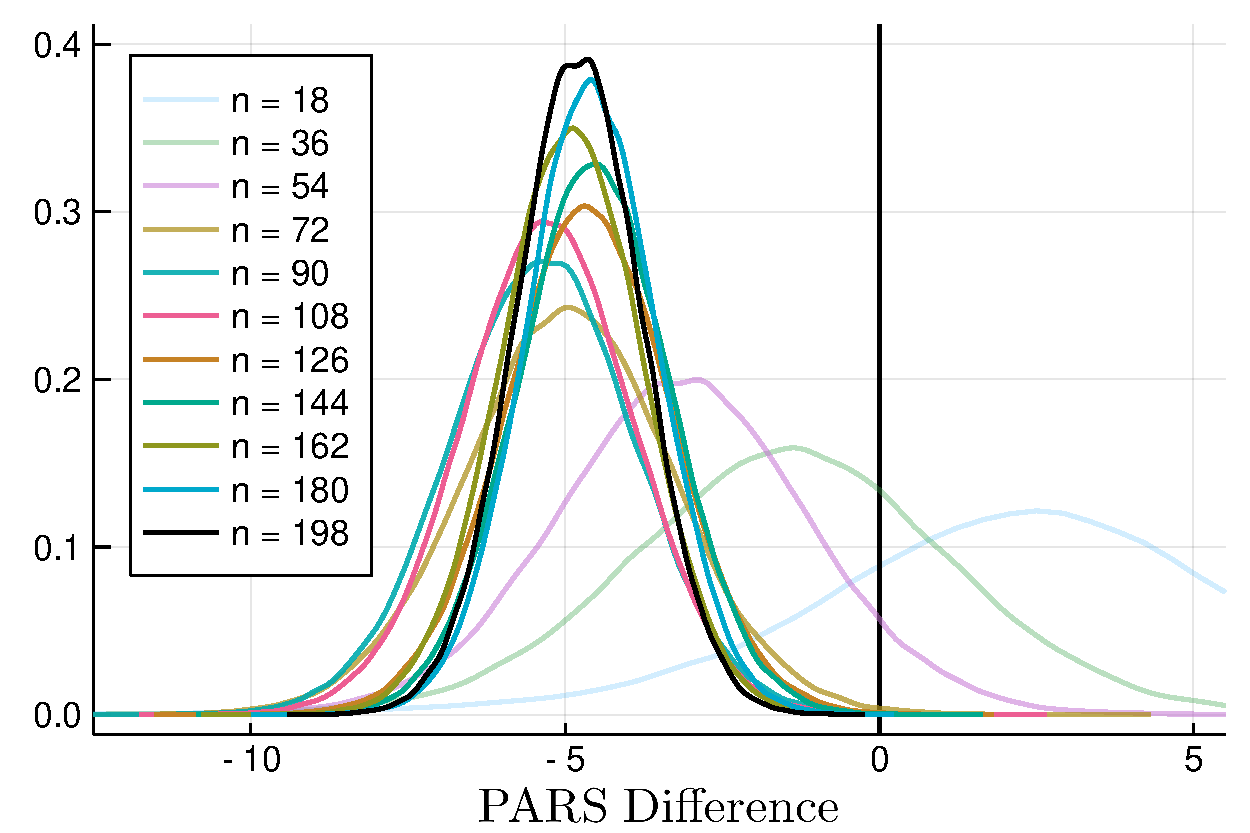
\includegraphics[width=8cm]{sequential_plot.pdf}}
	\caption{Difference in ATE between treatment and placebo groups.} 
	\label{fig:pars_diff}
\end{figure}

\begin{table}
	\tbl{Evidence Against $H_0$:$\delta=0$}{
		\begin{tabular}{rrrr} %\hline
			$n$   & $PDR(\delta = 0)$ & P$(\delta \ge 0)$ & $p$-value \\
			18  & 1.37       & 0.2382      & 0.4763  \\
			36  & 1.19       & 0.2887      & 0.5775  \\
			54  & 3.49       & 0.0625      & 0.1250  \\
			72  & 61.35      & 0.0025      & 0.0051  \\
			90  & 572.96     & 0.0003      & 0.0005  \\
			108 & 1083.5    & 0.0001       & 0.0002  \\
			126 & 329.24     & 0.0005      & 0.0010  \\
			144 & 610.67     & 0.0002      & 0.0004  \\
			162 & 4596.8    & 0.0000       & 0.0000   \\
			180 & 2394.6    & 0.0000       & 0.0000   \\
			198 & 46452.9   & 0.0000       & 0.0000    
	\end{tabular}}
	\label{tab:seq}
\end{table}
\vskip 6pt
There is clear evidence of a difference between SRT+CBT and PBO, $\delta$, by $n=72$ (posterior odds against $H_0$:$\delta=0.0$ are $61.4$:$1$, $P(\delta \ge 0|s,n) = 0.0025$,), suggesting that for this treatment comparison the clinical trial could have been completed with less than half of the original sample with no change in the conclusions.

\section{Bayesian hierarchical modeling}
\label{sec:hbm}

\begin{figure*}[t]
	\centerline{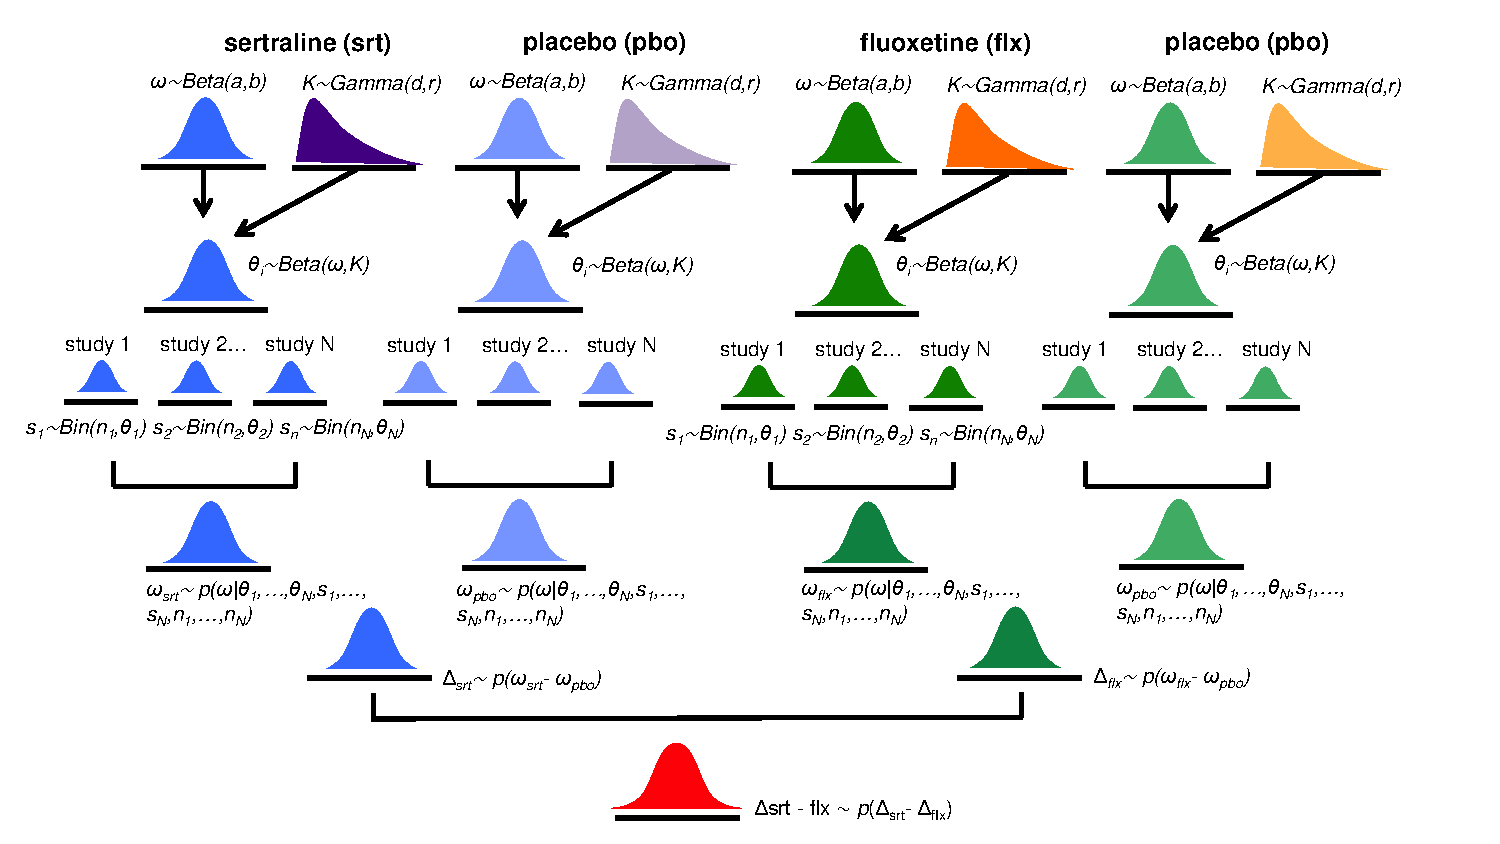
\includegraphics[width=18cm]{bhm_model.pdf}}
	\caption{Bayesian Hierarchical Model for Treatment Comparisons.}
	\label{fig:bhm}
\end{figure*}

A Bayesian hierarchical model (BHM) provides a flexible setting for modeling data that allows for heterogeneity across individuals or groups. If homogeneity across studies is assumed, the data can be combined via Bayesian updating as in the sequential analysis in the previous section.  For categorical data, all that is needed are the number of occurrences, $s_i$, in $n_i$ subjects in each study, $i$, of $N$ studies. The posterior distribution is then 
%\begin{equation}
%\begin{split}
%p(\theta | s_1,...,s_N, n_1,...,n_N,a,b) = \\ \textnormal{Beta}(\sum_{i=1}^N s_i %+a,\sum_{i=1}^N(n_i - s_i) + b),
%\end{split}
%\label{eq:pbeta}
%\end{equation}
\begin{equation}
%\begin{split}
p(\theta | s, n,a,b) = \\ \textnormal{Beta}( s + a, n - s + b),
%\end{split}
\label{eq:pbeta}
\end{equation}
where $s = \sum_{i=1}^N s_i$ and $n = \sum_{i=1}^N n_i$, with $a=b=1$ for a uniform prior for $\theta$.
\vskip 6pt
Alternatively, BHMs can allow for heterogeneity across studies due to different trial sites, different treatments, such as different medications, etc., and the same Bayesian machinery can be employed to compare a variety of treatments relative to placebo. For the categorical data examined herein there are two common BHM specifications: the Beta-Gamma\cite{Kruschke2014}, and the Logistic-Normal\cite{Mcelreath2015}.  In the following, we adopted the Beta-Gamma BHM specification as it directly provides intuitively understandable parameter estimates, whereas the logistic specification is more difficult to interpret (though is better suited when covariates are included).
\vskip 6pt
The complete Beta-Gamma BHM modeling framework is illustrated in Figure \ref{fig:bhm} for the case of comparing two sets of RCTs for different treatments (sertraline vs. fluoxetine) with placebo groups in each RCT. Each RCT in Figure \ref{fig:bhm} has a Binomial likelihood for $s_i$ successes in $n_i$ trials with probability of success $\theta_i$ (row 3).  A common Beta prior with mode $\omega$ and precision parameter $K$ is assigned to each $\theta_i$ (row 2), and a Beta and Gamma hierarchical prior are assigned to $\omega$ and $K$ respectively (row 1). The hyperparameters $a,b,d$ and $r$ are selected to represent a priori knowledge about the distributions of $\omega$ and $K$ (relatively uninformative priors are usually assigned unless other information is available).
\vskip 6pt
The package Turing.jl provides Hamiltonian Monte Carlo (HMC) and MCMC algorithms to obtain posterior density MCMC chains from an large variety of models. The Julia macros provide a flexible and intuitive modeling and inference framework. The model specification in Turing.jl closely matches how one would write the model mathematically, e.g. for the Beta-Gamma BHM (Turing code examples for the Logistic-Normal are available at github.com/TuringLang/Turing.jl and github.com/StatisticalRethinkingJulia):
\begin{lstlisting}[language = Julia]
using Turing, MCMCChains
@model binomial_trials(s,n) = begin
	g = length(n)  # number of groups
	# hierarchical priors
	ω ~ Beta(2,3)
	K ~ Gamma(10,1/0.05)
	a = ω*K + 1.0
	b = (1.0 - ω)*K + 1.0
	# priors for each occurrence rate
	θ = Array{Real}(undef, g)
	for k in 1:g
		θ[k] ~ Beta(a,b)
	end
	# likelihood
	for i in 1:g
		s[i] ~ Binomial(n[i],θ[i])
	end
end
\end{lstlisting}

A few more lines of code provide posterior samples from the No U-Turn (NUTS) sampler in Turing.jl, allowing evaluation of the no mean difference between two groups hypothesis:
\begin{lstlisting}[language = Julia]
using BayesTesting

# treatment
ctrt = mapreduce(c->sample(binomial_trials(s2, n2),
	NUTS(5000,1000,0.65)),chainscat,  1:5)
# placebo
cpbo = mapreduce(c->sample(binomial_trials(s1, n1),
	NUTS(5000,1000,0.65)), chainscat,  1:3)

ωₜ = Array(ctrt["ω"][1001:end])  # treatment ω
ωₚ = Array(cpbo["ω"][1001:end])  # placebo ω
δ = ωₜ - ωₚ           # difference
plot(δ,st=:density,label="Difference")

# compute summary stats, PDR odds, tail prob.
[mean(δ) std(δ)]
quantile(δ,[0.025,0.5,0.975])
[mcodds(δ, h0=0.0) bayespval(δ)]
\end{lstlisting}

In recent work\cite{Mills2019b}, a meta-analysis of results from several RCTs was conducted to obtain more complete evidence on the expected side effects of SSRIs.  Side effect or adverse event (AE) occurrence in an RCT is generally recorded as a categorical variable, leading to binomial data consisting of number of AEs, $s_i$, in $n_i$ subjects for trial $i$. The results below are for the  “activation” (or restlessness) AE.  Five studies included data for activation.  Posteriors for each of the five studies for treatment (with SSRI) and placebo were obtained using Turing.jl (the third row of distributions in Figure~\ref{fig:bhm}), along with the distribution of the mode, $\omega$, of the posterior for the estimated rate of success for each study, $\theta_i$ (the fourth row in the Figure~\ref{fig:bhm}).  Given the MCMC pseudo-samples for each $\omega$ (e.g., SSRI-related side effects and placebo-associated side effects), outcome differences between treatment and placebo, then differences in differences between the two treatments relative to placebo (e.g. SSRI vs. SNRI-related side effects) can be determined (rows 5 and 6 in the Figure~\ref{fig:bhm}).
\vskip 6pt

Using the NUTS sampler in Turing.jl, the BHM was estimated for each treatment arm of the study data. Run times to generate 5 chains using the above code were approx. 7 seconds or less on a laptop with CPU: Intel(R) Core(TM) i7-6600U CPU @ 2.60GHz running Julia Version 1.1.0. The stability of the chains and similarity of each chain density suggests convergence to the marginal posteriors has been attained, as illustrated in Figure~\ref{fig:chains}.
\begin{figure}[t]
%	\centerline{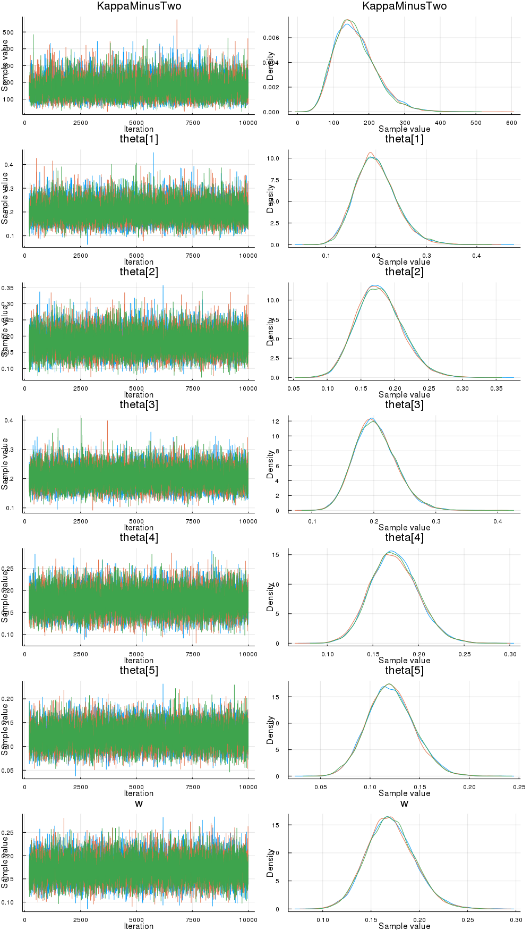
\includegraphics[width=8cm]{mc_chains.png}}
	\centerline{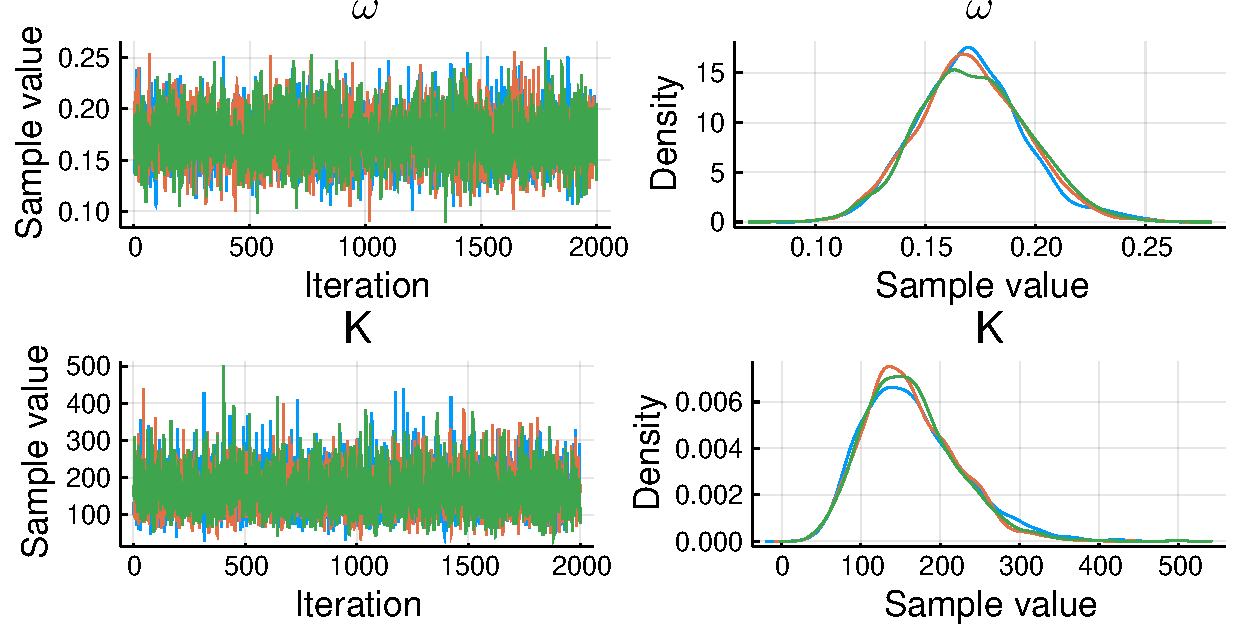
\includegraphics[width=8cm]{omega_K_mcmcplot.pdf}}
	\caption{HMC chains from No U-Turn Sampler.}
	\label{fig:chains}
	\end{figure}

The resulting posterior densities for each study probability of occurrence rate (risk), $\theta_j$ and the hierarchical probability of occurrence across groups, $\omega$ are illustrated in Figure~\ref{fig:activ}. Results using the logistic-normal specification gave very similar results. The results for activation due to SSRI (mean difference between treatment and placebo, $\delta$), given in Figure~\ref{fig:diff} and Table~\ref{tab:delta_results}, provide statistical evidence of an increased likelihood of activation with the treatment. To examine the impact of across study heterogeneity, Figure~\ref{fig:compare} presents the BHM posterior density for $\omega$ in comparison to combining all studies ignoring across study heterogeneity via equation~(\ref{eq:pbeta}).

% activation_posteriors.png
\begin{figure}[t]
	\centerline{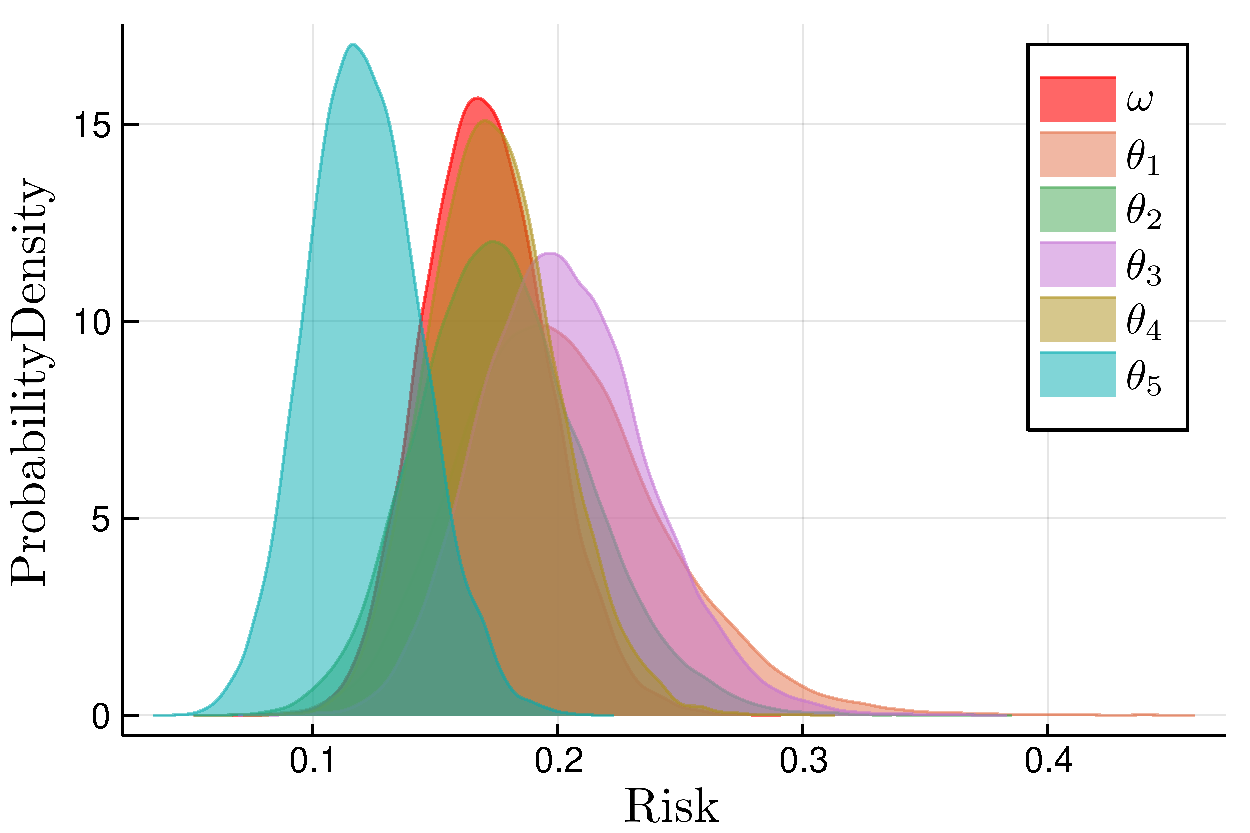
\includegraphics[width=8cm]{thetas_omega.pdf}}
	\caption{Posterior Densities for Activation}
	\label{fig:activ}
\end{figure}

\begin{figure}[t]
	\centerline{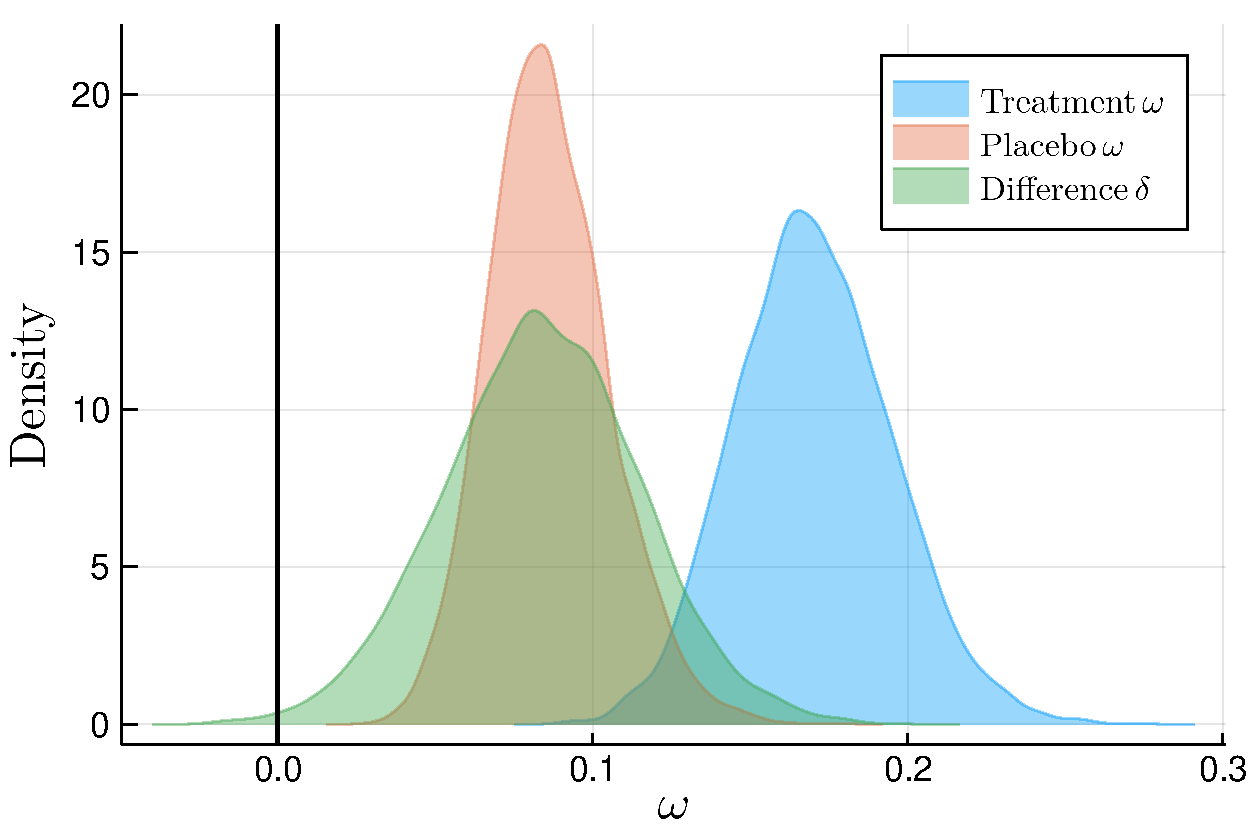
\includegraphics[width=8cm]{treat_pbo_diff2.pdf}}
	\caption{Treatment-Placebo Difference}
	\label{fig:diff}
\end{figure}


\begin{table}
		\tbl{Posterior difference in treatment and placebo, $\delta$}{
	\begin{tabular}{cccccc}
		mean  & SD    & $PDR(\delta = 0)$   & P$(\delta \le 0)$ & \multicolumn{2}{c}{0.95 CrI} \\
		0.084 & 0.031 & 35.75 & 0.003   & 0.023         & 0.145       
	\end{tabular}}
	\label{tab:delta_results}
\end{table}


% bhm_vs_non_compare.png
\begin{figure}[t]
	\centerline{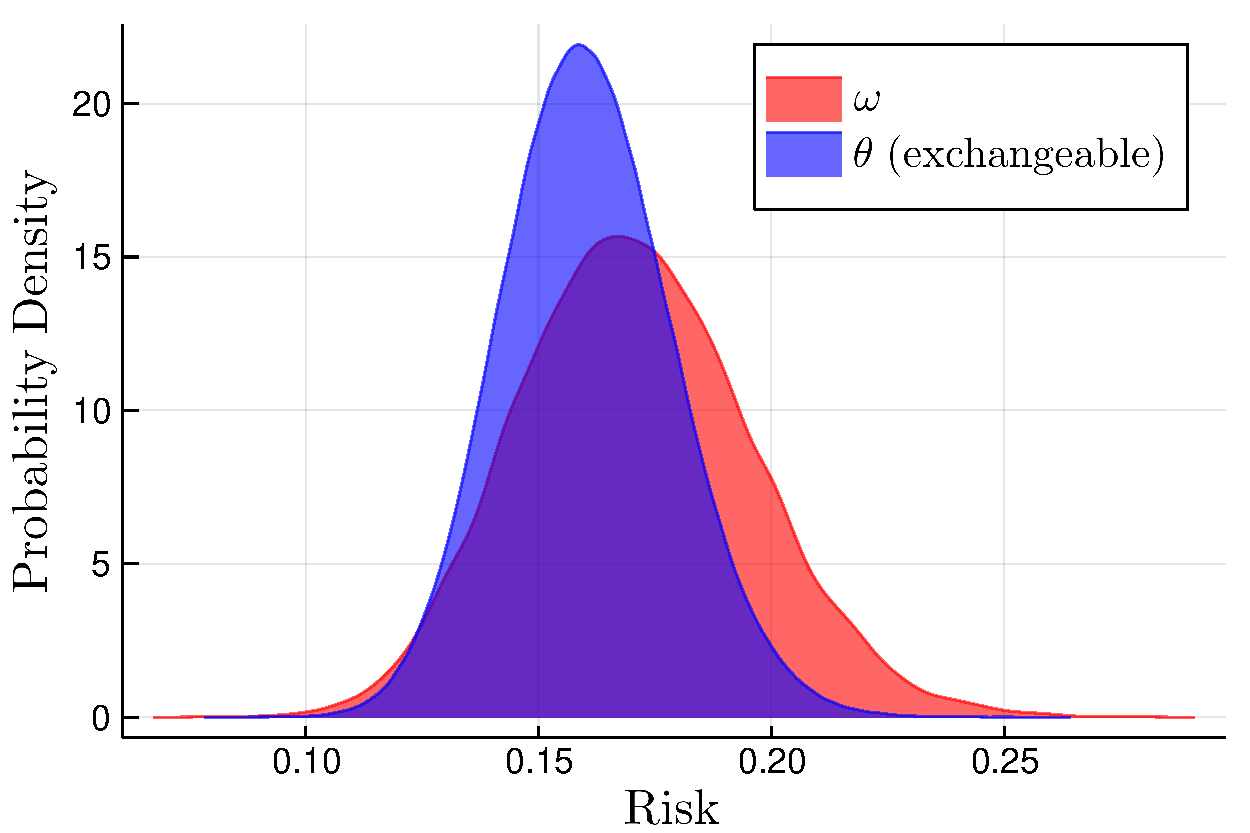
\includegraphics[width=8cm]{bhm_vs_exc.pdf}}
	\caption{ATE posterior density with and without heterogeneity}
	\label{fig:compare}	
\end{figure}
 
\section{Summary and Conclusions}
This paper presented two examples of application of Bayesian probabilistic modeling from our research that illustrate our experiences with Bayesian inferential methods for clinical research using Julia.  We have used this approach in several studies including: reevaluating the evidence from previously conducted RCTs; analysis of abandoned trials; joint evaluation of tolerability and efficacy in RCTs; and BHMs for meta-analysis evaluating adverse events (“side effects”) in trial participants.
\vskip 6pt
The approach presented provides a solution to the strong institutional inertia of `$\le 5\% =$ statistical significant’ through provision of PDRs (or `posterior odds') as well as posterior tail probabilities (`Bayesian $p$-values’), posterior density intervals, and visualization of posterior densities. This allows for more flexibility in the choice of critical value for a particular test, i.e. the cut-off point for rejecting vs. failing to reject the null hypothesis.  For example, researchers at CERN attempting to detect gravitational waves would wish to employ a much larger critical odds ratio (akin to the `5-sigma rule'), whereas researchers comparing the efficacy of two relatively harmless psychiatric treatments for anxiety or depression would undoubtedly find posterior odds that pass a much lower critical threshold convincing enough to recommend one treatment over another.  
\vskip 6pt
One of the major advantages of the contemporaneous Bayesian approach is 
its ability to utilize MC and MCMC methods. This approach is computationally intensive, but less mathematically and analytically burdensome. Moreover, it typically requires fewer restrictions than needed for analytical tractability.  We find Julia to be ideal for scientific programming of this nature; it reduces the need for the researcher to wear multiple expertise `hats'. The resulting conservation of clinical researchers' time and energy by using Julia is substantial, and allows greater focus on the scientific and clinical problems. Ultimately, this potentially hastens the arrival of effective treatments and findings to the clinic.

\bibliographystyle{juliacon}
\bibliography{ref}
%\end{verbatim}
%When submitting the document source (.tex) file to external
%parties, the ref.bib file should be sent with it.
%\cite{bezanson2017julia}

%% **************GENERATED FILE, DO NOT EDIT**************

\bibliographystyle{juliacon}
\bibliography{ref.bib}

\end{document}

% Inspired by the International Journal of Computer Applications template